%% preliminaries.tex
%%

%% ==============
\chapter{Preliminaries}
\label{ch:preliminaries}
%% ==============

In this chapter we shall provide an overview of the definitions and structures used in this thesis.

\section{Definitions}

A \textit{Graph} is defined as a tuple of a set of nodes and a set of edges, connecting these nodes, commonly denoted as $G \defines (V, E)$, with $V$ being the nodes and $E$ being the edges.

In a \textit{Directed Graph}, the edges itself are represented by tuples of nodes in the form of $(u,v)\in E$ and $u, v \in V$ respectively, which means that there is an outgoing edge from node $u$ pointing to node $v$. A bidirectional graph uses sets as edges instead, as the order of the edges doesn't matter in that case.

A \textit{Subgraph} of a graph $G$ contains a subset of $G$'s nodes and edges, and being a graph itself, of course doesn't contain any edges that do not connect to nodes. As a shorthand for declaring a subgraph $S \subseteq G = (V, E)$ using a subset of its nodes $U \subseteq V$, we will be writing $S = (U, E(U))$, where $E(U) \defines \{(u,v)\in E : u,v\in U\}$.

For directed graphs, we define its \textit{Degree} as the maximum in-degree of its nodes, which means the biggest number of edges connecting towards any one node in that graph, and commonly refer to it by the letter $\Delta$.

A \textit{Node Coloring} is a function $\varphi : V \rightarrow \mathbb{N}$ that assigns each node $v\in V$ a color, usually represented by natural numbers. A node coloring is \textit{legal} or \textit{valid} if for every edge $(u, v)\in E$, $\varphi (u) \neq \varphi (v)$.

In the context of the following algorithms, the symbol $[x]$ with $x \in \mathbb{N}$ is defined as the set $\{1, 2, \dots , x\}$, and might be referred to as \textit{Pool}, as it contains all colors up to $x$.

\section{The Communication Model}\label{section:comm}

Throughout this thesis we will work with the CONGEST communication model. This abstracts the actual message transmission away from our algorithms and our algorithms use the notion of communication rounds instead of a common clock to slice time, this is a slightly more abstracted model, but we can still run our algorithms in the SINR model using local broadcasting.

One round of communication involves a node $v$ sending a message of length at most $O(\log n)$ (as any meaningful communication involves at least the id of a node) to all of its outgoing neighbors $u$ ( $(v, u) \in E$ ), and receiving one message from all incoming edges $(u, v) \in E$. Transmitting a message of a length dependent on an asymptotically larger factor $\gamma$ will then be equivalent to $O(\log n + \gamma)$ rounds of normal messages to be delivered.

There are many different algorithms to produce this type of unstructured message passing, which we may also call a local broadcast. For example, in the SINR model with fixed transmission ranges, a local broadcast round takes $O(\Delta \cdot (\log n + \gamma))$ timeslots to pass a message of length $\gamma$ with high probability to all neighbors, given that the maximum degree $\Delta$ is known \cite{dt-dncsi-10}. 

The motivation for the directed graph analysis in this thesis however came from the SINR model using variable transmission power. We generally assume that the maximum degree $\Delta$ is known throughout this thesis, and with that parameter known, a local broadcast takes $O(\Gamma^{2} \Delta \log n)$ timeslots to transmit the messages with high probability, with $\Gamma$ being the ratio between the maximal and the minimal transmission ranges \cite{DBLP:journals/corr/FuchsW14}. 

Research is currently being done to move towards a fully realistic model using signal decay, which generalises the SINR model \cite{DBLP:journals/corr/BodlaenderH14}. At this point, however, there are no reliable local broadcasting algorithms adapted to this model yet, however if and when such an algorithm is found, it would then enable the algorithms from this thesis to work on that model, as well.

\section{Graph Model Characterization}\label{section:graph}

To create our communication graph, we take a look at the SINR communication model with arbitrary transmission power. This results in each node having an arbitrary transmission range and hence, a node with a larger transmission range could send messages to nodes with lower transmission ranges, which cannot answer. This results in a disk graph of arbitrary disk sizes.

\begin{figure}[ht]
\center
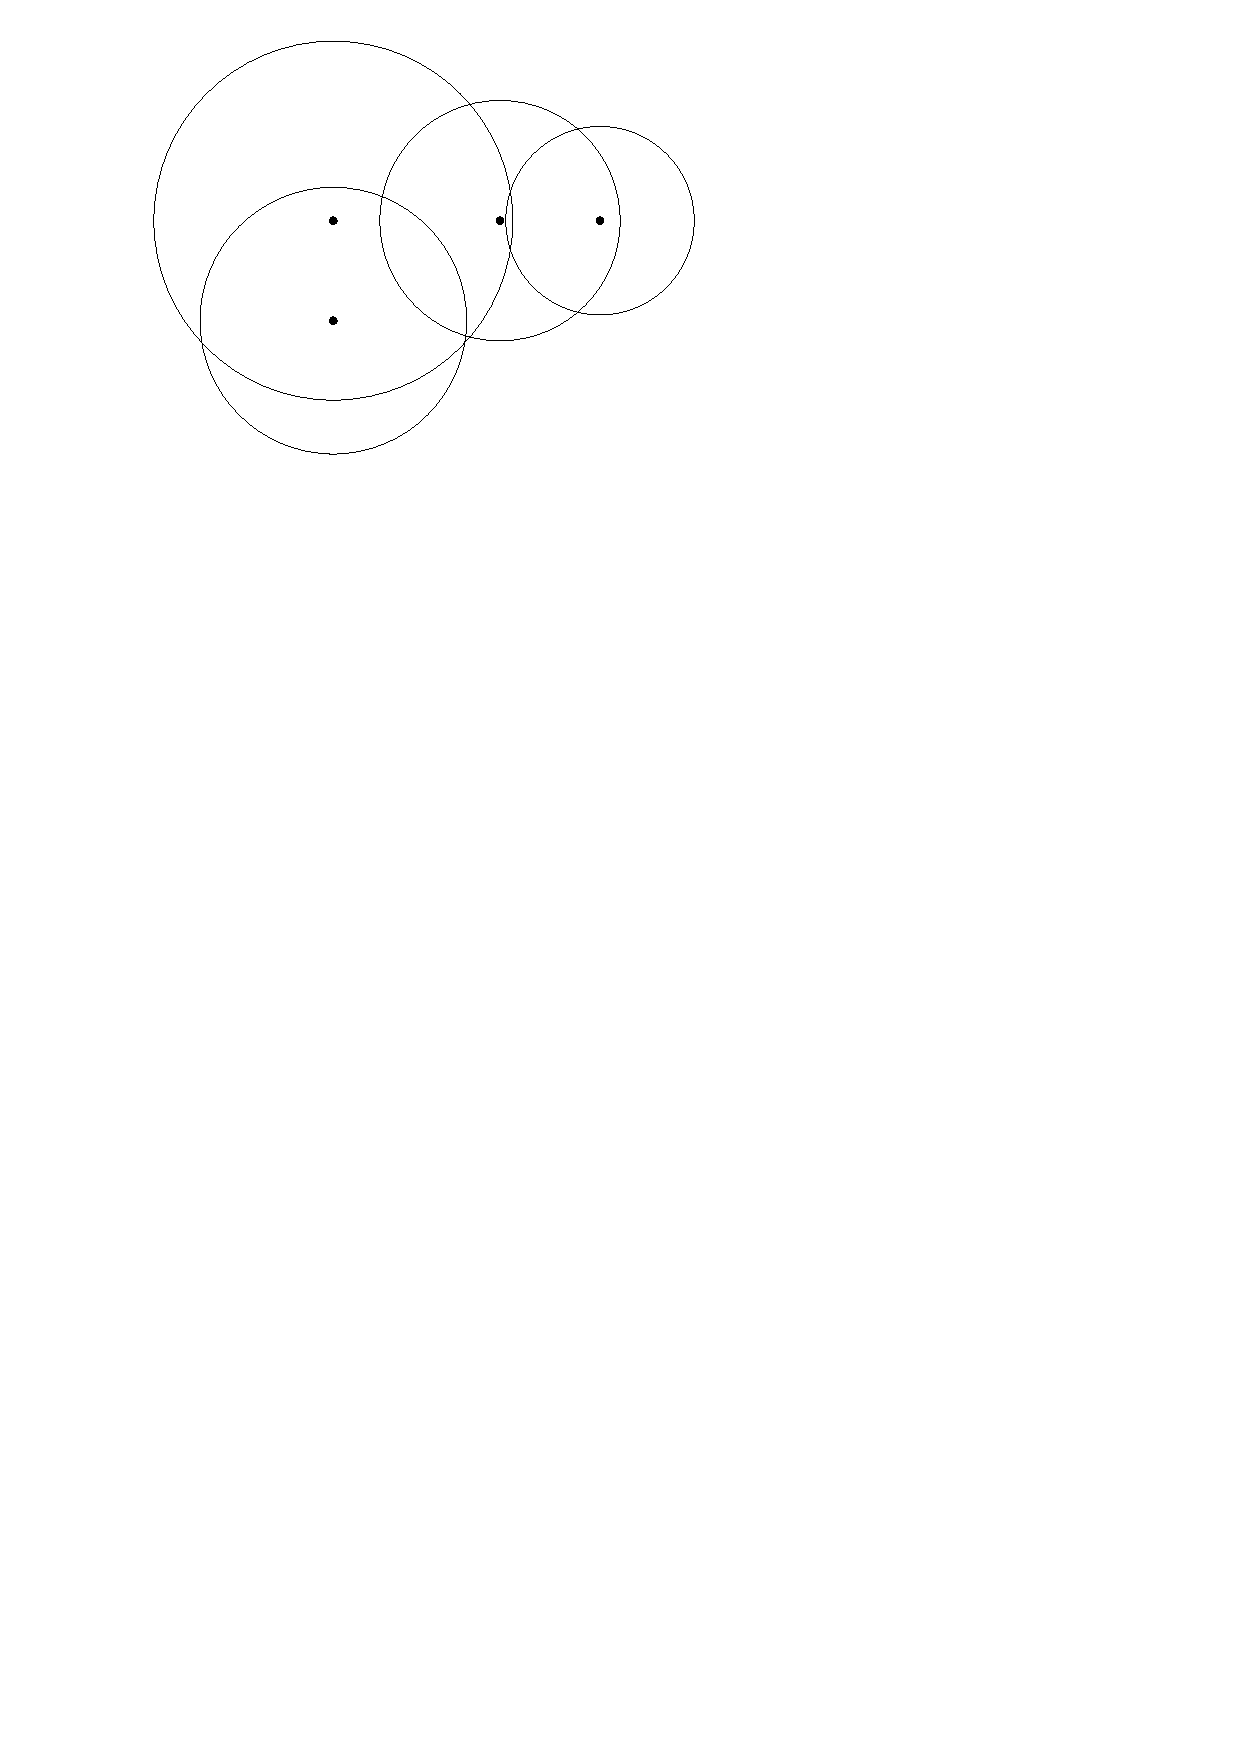
\includegraphics[scale=0.7]{figures/transmissionrange.pdf}
\caption{Four nodes with different transmission ranges\label{figure:tr}}
\end{figure}
\begin{figure}[ht]
\center
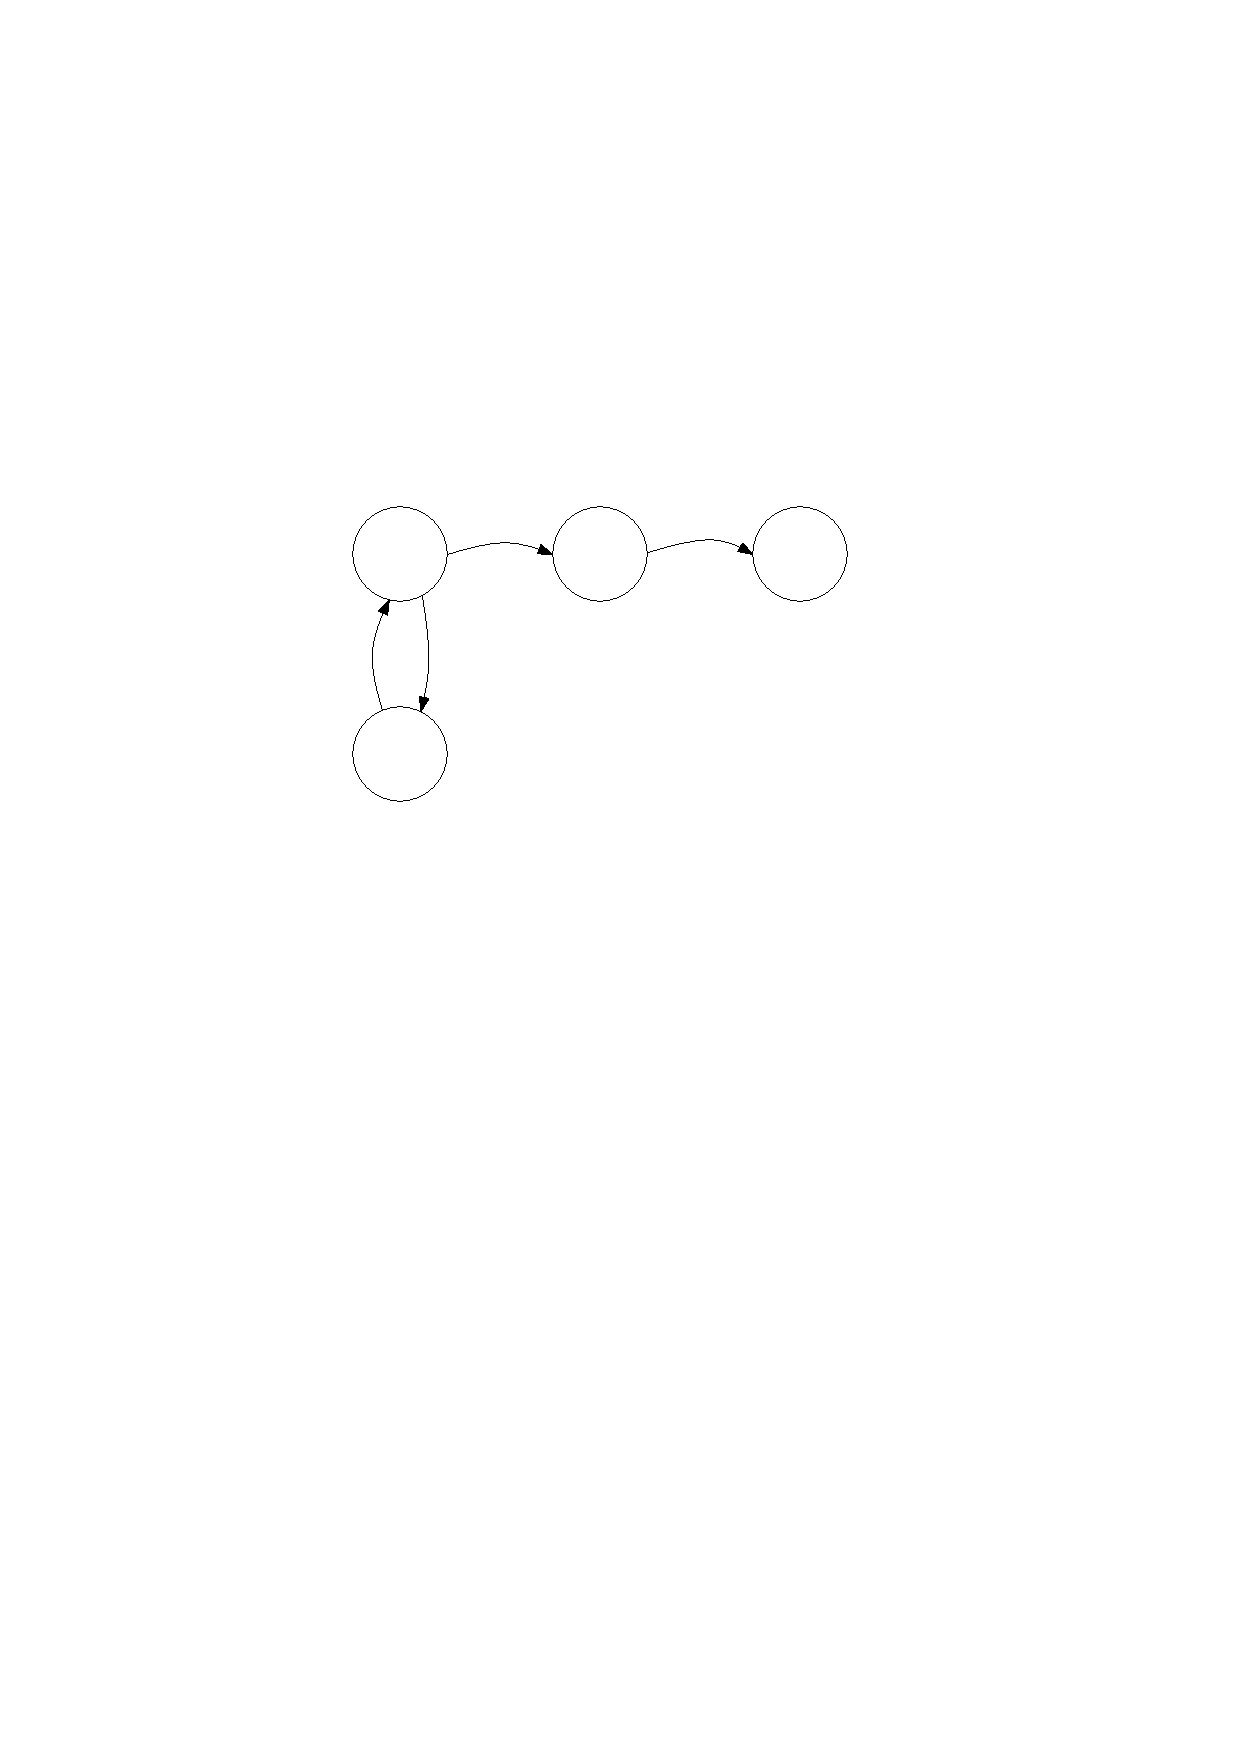
\includegraphics[scale=0.7]{figures/resultinggraph.pdf}
\caption{The communication graph resulting from Figure~\ref{figure:tr}}
\end{figure}


A \textit{Cycle} is defined as a finite set of edges $C \subseteq E$ so that you can construct a simple path $(u, v, \dots, u)$ from any starting edge $\in C$. Any bidirectional communication in our graph model is a cycle of length 2. Additionally we will introduce \textit{Strictly Directed Cycles}. These are cycles defined as before with an additional restriction: for any edge $(v, u) \in C$ it must hold that $(u, v) \notin E$.

\begin{lemma}
	In a disk graph, there are no strictly directed cycles.
\end{lemma}
\begin{proof}
	A strictly directed path $(u, v, \dots, w)$ implies that the transmission range $T_r(v)$ of each following node is smaller than the range of the node before it:
	$T_r(u)>T_r(v)>\dots>T_r(w)$. A cycle implies that the last node equals the first node ($u=w$), which would result in $T_r(u) > T_r(u)$ which is obviously impossible.
\end{proof}


\begin{figure}[ht]
\center
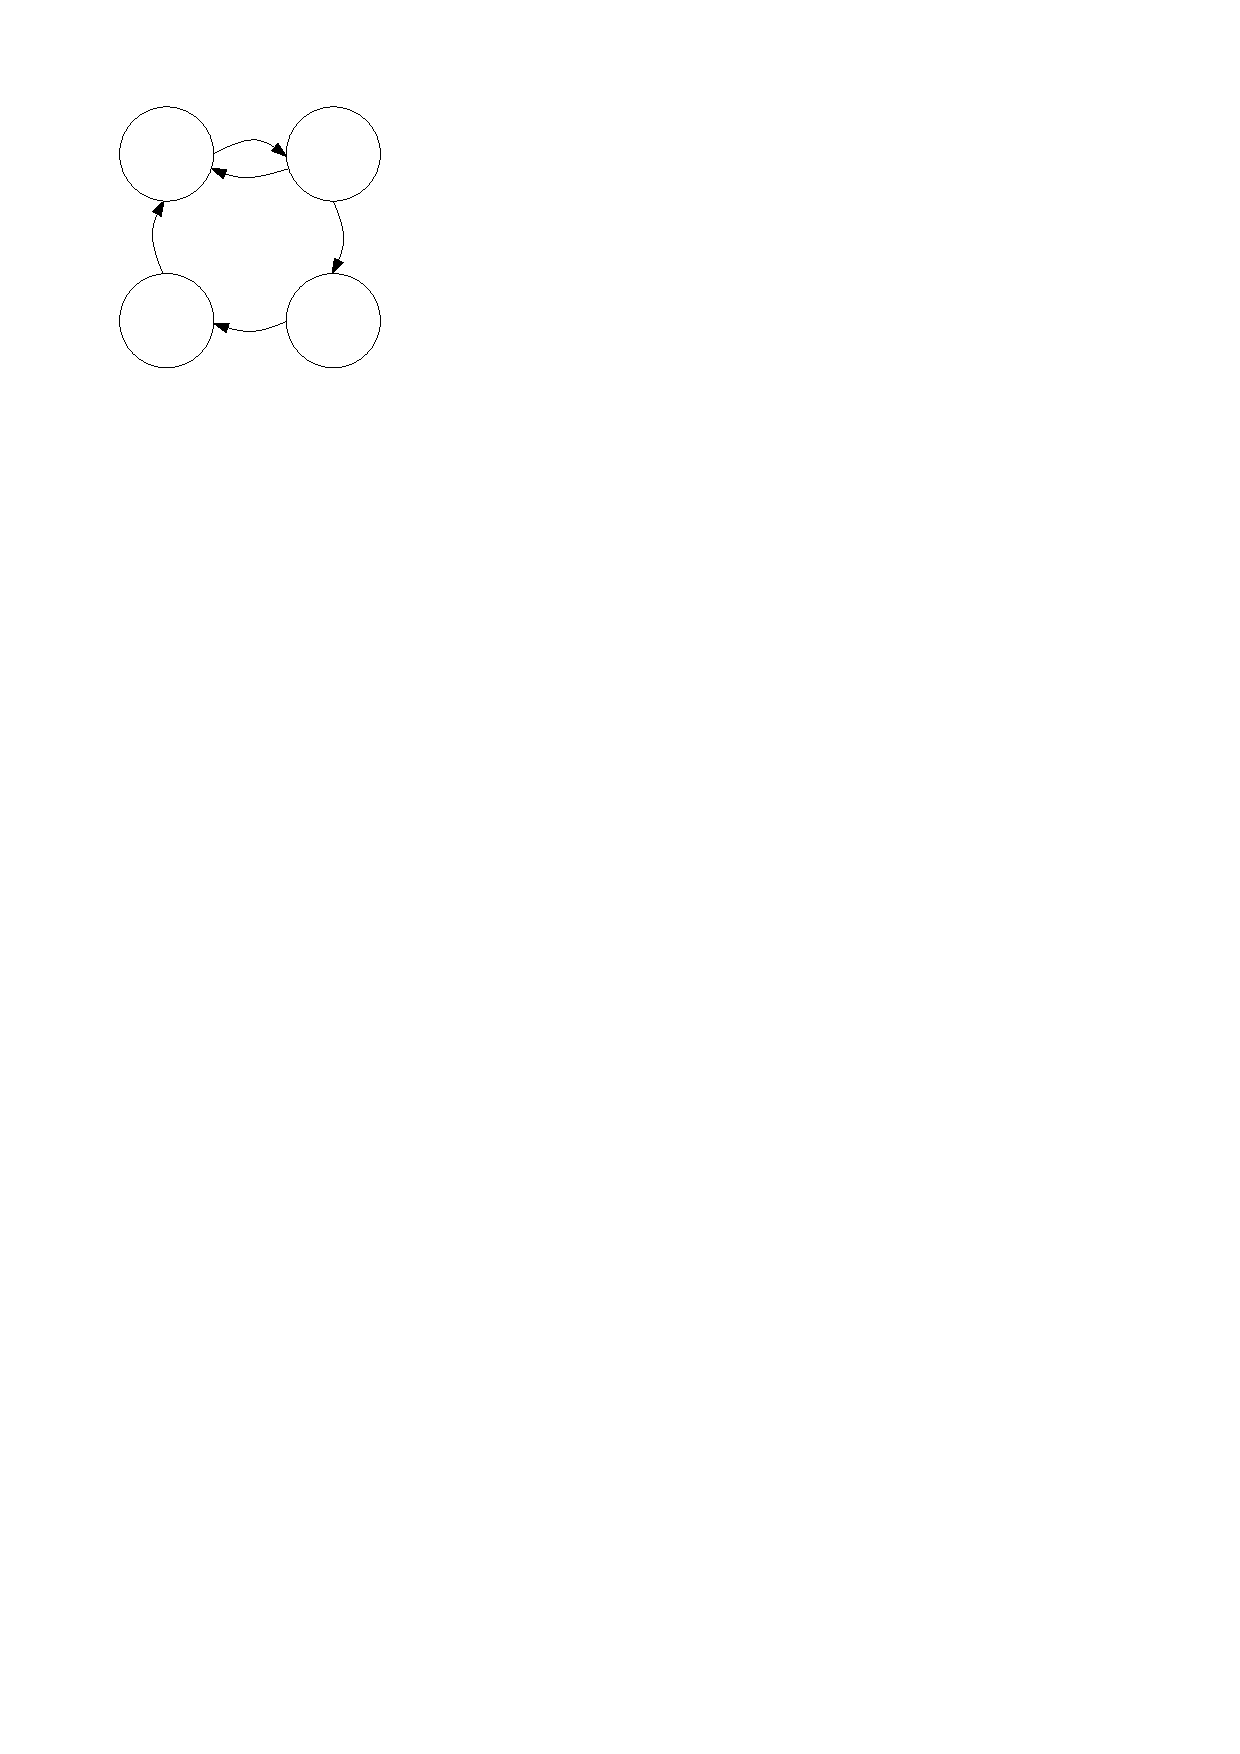
\includegraphics[width=0.2\linewidth]{figures/normalcycle.pdf}%
\hspace{2cm}
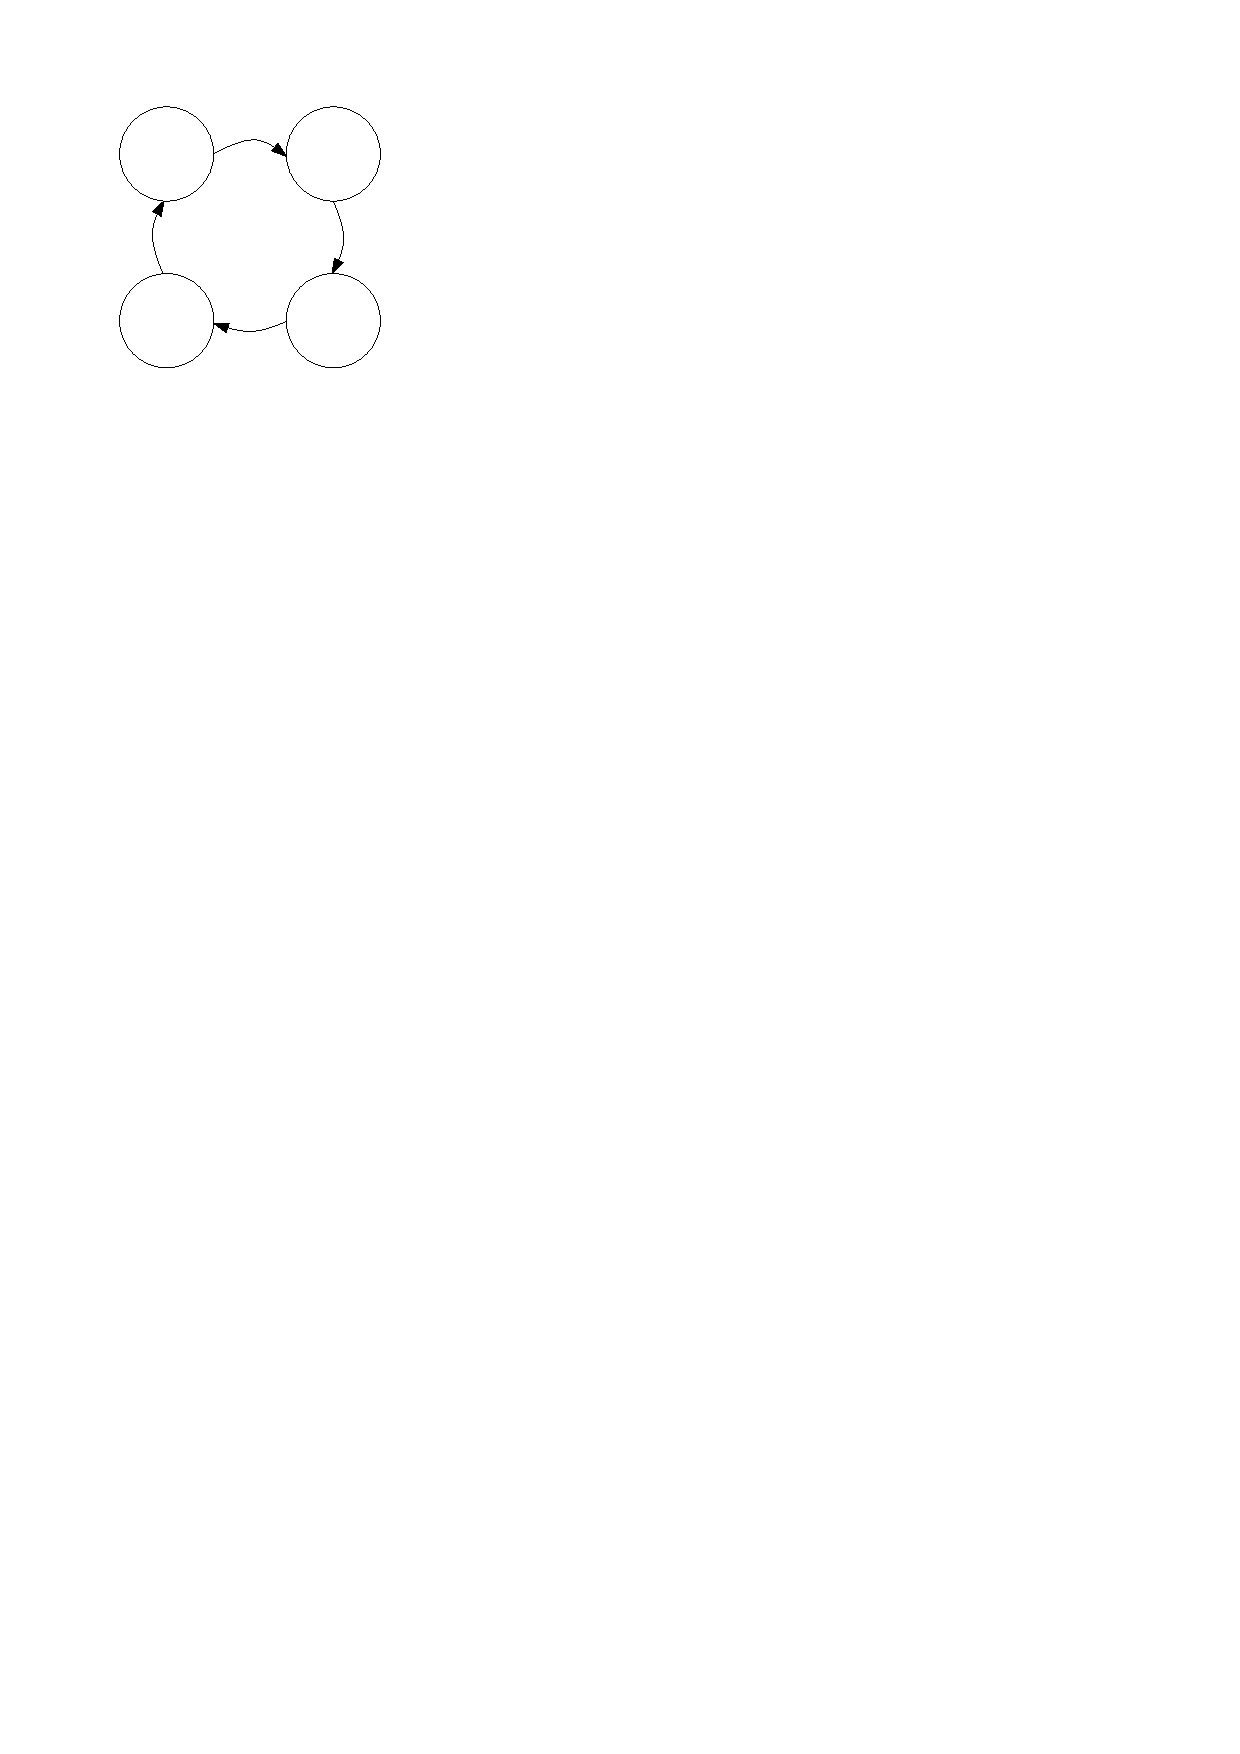
\includegraphics[width=0.2\linewidth]{figures/strictlydirectedcycle.pdf}%
\caption{Left: Graph containing two cycles, yet no strictly directed cycle. \\Right: Graph containing one strictly directed cycle.}%
\end{figure}

As these directed cycles are not possible in this model, we will work with the assumption that they do not exist in this thesis. However, in reality, this scenario could occur. At the end of the thesis, we will discuss the implications of these cycles on our algorithms.

One parameter which will be used often throughout this thesis is the parameter $l$, which describes the length of the longest strictly directed path $P$: $l = |P|+1$. This parameter, which is essentially 1 in unit disk graphs, influences the runtime of algorithms in this model, as we show in the proof of Algorithm~\ref{alg:r2d}.